\section{Results}
The first model, shown in Figure \ref{fig:ESN1}, we trained with 1000 hours of
historical data. The blue line is a snapshot of historical demand data. The
dashed line indicates the end of the model training and the beginning of the
model prediction. The red line is the prediction made by the \gls{ESN}. By
inspection, the \gls{ESN} successfully predicted a general
trend but had difficulty with accuracy at the desired hourly resolution.

\begin{figure}[h]
  \centering
  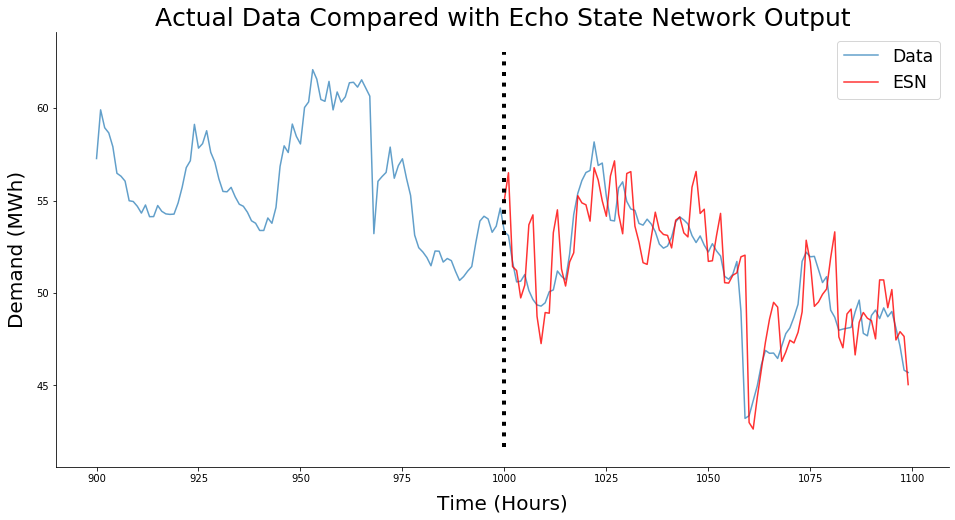
\includegraphics[width=\columnwidth]{scaled_esn_network2.png}
  \caption{A simple ESN with a prediction of 100 hours into the future after
  training on 1000 hours of historical data.}
  \label{fig:ESN1}
\end{figure}

The second model, shown in Figure \ref{fig:ESN2}, we trained with the same
dataset as before and extended the training to 3500 hours of
historical data. This \gls{ESN} made better predictions than the first model
and is most likely due to longer training. The effect of training
length on model accuracy will be explored in future work.

\begin{figure}[h]
  \centering
  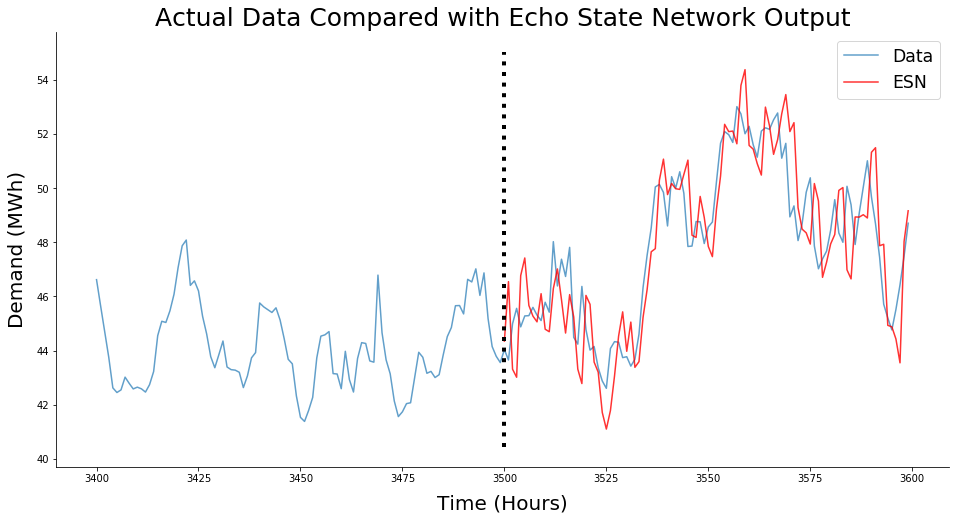
\includegraphics[width=\columnwidth]{scaled_esn_network.png}
  \caption{A simple ESN with a prediction of 100 hours into the future. After
  training on 3500 hours of historical data.}
  \label{fig:ESN2}
\end{figure}

Both models use training data with an hourly resolution. It is possible
that data at the 15-minute or 30-minute timescale will improve prediction
accuracy.
